
\section{AWGN channel} 
\subsection{Introduction} 
\begin{frame}{Decoder for an AWGN channel}
In the Tanner graph, the bit nodes are called repetition nodes and the check nodes are called zero-sum nodes. The incoming information at each bit node corresponds to that single variable only, which is the same case as a repetition code and the . The incoming information at each check node corresponds to the parity check constraint, which is also called as zero-sum constraint.\newline

So, we split the belief propagation decoder into two parts - SISO (soft-input-soft output) decoder for a repetition code and SISO decoder for SPC (Single Parity Check) code.
\end{frame}

\subsection{SISO decoder for Repetition code} 
\begin{frame}{SISO decoder for Repetition code}
Consider a (3, 1) repetition codeblock $(c_1, c_2, c_3)$.\\
Let $L_i$ = "belief" that $c_i = 0$. \\
Output of the decoder: intrinsic + extrinsic \\
\begin{block}{\underline{Intrinsic belief (Log-likelihood ratio)}:}
\end{block}
\begin{gather*}
    Pr(c_1 = 0 | r_1) = \frac{f(r_1|c_1 = 0) Pr(c_1 = 0)}{f(r_1)} \\
    Pr(c_1 = 1 | r_1) = \frac{f(r_1|c_1 = 1) Pr(c_1 = 1)}{f(r_1)}
\end{gather*}

We are using BPSK modulation scheme.  If $ c_1 = 0$, symbol = +1. \\ $ \Rightarrow r_1 = 1 + \mathcal{N}(0, \sigma ^2)$ \\
Similarly, if $ c_1 = 1$, symbol = -1. \\ $ \Rightarrow r_1 = -1 + \mathcal{N}(0, \sigma ^2)$
\end{frame}
\begin{frame}{SISO decoder for Repetition code (contd...)}

\begin{gather*}
\text{Likelihood ratio} : \frac{Pr(c_1 = 0|r_1)}{Pr(c_1 = 1|r_1)} =  \frac{f(r_1|c_1 = 0)}{f(r_1|c_1 = 1)} \\
\Rightarrow \frac{Pr(c_1 = 0|r_1)}{Pr(c_1 = 1|r_1)} = \frac{\frac{1}{\sqrt{2 \pi \sigma ^ 2}} \exp(\frac{{(r_1-1)}^2}{2 \sigma ^2})}{\frac{1}{\sqrt{2 \pi \sigma ^ 2}} \exp(\frac{{(r_1+1)}^2}{2 \sigma ^2})}
= \exp({\frac{2r_1}{\sigma ^2}})
\end{gather*}
\begin{gather*}
\begin{split}
\text{Log-Likelihood ratio} :log \left(\frac{Pr(c_1 = 0|r_1)}{Pr(c_1 = 1|r_1)} \right) & = \frac{2r_1}{\sigma ^2} \\
& = r_1 \times constant
\end{split}
\end{gather*}
Generally, the constant is ignored. This LLR is called intrinsic LLR (or input LLR or channel LLR) 
\end{frame}

\begin{frame}{SISO decoder for Repetition code (contd...)}
\begin{exampleblock}{\underline{Output LLR}:}
\end{exampleblock}
\begin{gather*}
L_i = log \left(\frac{Pr(c_i = 0|r_1, r_2, r_3)}{Pr(c_i = 1|r_1, r_2, r_3)} \right) \\
L_1: \frac{Pr(c_1 = 0|r_1, r_2, r_3)}{Pr(c_1 = 1|r_1, r_2, r_3)} = \frac{f(r_1r_2r_3|c_1 = 0)}{f(r_1r_2r_3|c_1 = 1)}
\end{gather*}
Suppose $c_1 = 0 \Rightarrow \text{ symbol vector} = [+1, +1, +1]$
\begin{gather*}
    r_1 = 1 + \mathcal{N}_1(0, \sigma ^2)\\
    r_2 = 1 + \mathcal{N}_2(0, \sigma ^2)\\
    r_3 = 1 + \mathcal{N}_3(0, \sigma ^2),
\end{gather*}
where $\mathcal{N}_1, \mathcal{N}_2, \mathcal{N}_3$ are i.i.d.

\end{frame}

\begin{frame}{SISO decoder for Repetition code (contd...)}
\begin{gather*}
    \frac{Pr(c_1 = 0|r_1, r_2, r_3)}{Pr(c_1 = 1|r_1, r_2, r_3)} = \frac{\exp(\frac{{(r_1-1)}^2}{2 \sigma ^2}) \exp(\frac{{(r_2-1)}^2}{2 \sigma ^2}) \exp(\frac{{(r_3-1)}^2}{2 \sigma ^2})}{\exp(\frac{{(r_1+1)}^2}{2 \sigma ^2}) \exp(\frac{{(r_2+1)}^2}{2 \sigma ^2}) \exp(\frac{{(r_3+1)}^2}{2 \sigma ^2})} \\~\\
     = \exp(\frac{2(r_1+r_2+r_3)}{\sigma ^2})
\end{gather*} 
\begin{gather*}
    \Rightarrow L_1 = \frac{2(r_1+r_2+r_3)}{\sigma ^2} \\
   \Rightarrow L_1 \propto (r_1 + r_2 + r_3)
\end{gather*}
$r_1$ : Intrinsic belief, $r_2 + r_3$: Extrinsic belief 
\end{frame}


\subsection{SISO decoder for an SPC code}
\begin{frame}{SISO decoder for an SPC code}
Consider a general (n, n-1) SPC code.
If $\textbf{m} = [m_1, m_2,....., m_{n-1}]$, then the codeword $\textbf{c} = [c_1, c_2,....., c_{n-1}, p]$, where $p = m_1 \oplus m_2 \oplus ..... \oplus m_{n-1}$.

In an SPC codeword, the no. of 1's is even, due to the parity-check condition $c_1 \oplus c_2 ..... \oplus c_n = 0$. 

Suppose n = 3. Then, we have $c_1 = c_2 \oplus c_3$. 

Given $p_2 = Pr(c_2 = 0)$ and $p_3 = Pr(c_3 = 0)$, we need to find $p_1 = Pr(c_1 = 0|r_2, r_3)$. \\~\\

\begin{columns}[T,onlytextwidth]
\textbf{Truth table:}
\column{0.4\textwidth}
\begin{tabular}{cc|c}
$c_2$ & $c_3$ & $c_1$ \\
\hline
0 & 0 & 0 \\
1 & 1 & 0 \\
0 & 1 & 1 \\
1 & 0 & 1 \\
\end{tabular}

\column{0.4\textwidth}
From the truth table,
\begin{equation*}
    \begin{split}
        p_1  = p_2p_3 + (1-p_2)(1-p_3) \\
        1 - p_1  =  p_2(1-p_3) + (1-p_2)p_3
    \end{split}
\end{equation*}
\end{columns}
\end{frame}

\begin{frame}{SISO decoder for an SPC code (contd...)}
\begin{gather*}
    p_1 - (1-p_1) = p_2(p_3-(1-p_3)) + (1-p_2)((1-p_3)-p_3) \\~\\
    \frac{2p_1 - 1}{p_1 + 1 - p_1} = \frac{2p_2 - 1}{p_2 + 1 - p_2} \ \frac{2p_3 - 1}{p_3 + 1 - p_3} \\~\\
    \Rightarrow \frac{1-\frac{(1-p_1)}{p_1}}{1+\frac{(1-p_1)}{p_1}} = \frac{1-\frac{(1-p_2)}{p_2}}{1+\frac{(1-p_2)}{p_2}} \ \frac{1-\frac{(1-p_3)}{p_3}}{1+\frac{(1-p_3)}{p_3}} \\~\\
    \frac{1 - e^{-l_{ext, 1}}}{1 + e^{-l_{ext, 1}}} = \frac{1 - e^{-l_2}}{1 + e^{-l_{2}}} \frac{1 - e^{-l_3}}{1 + e^{-l_{3}}},
\end{gather*}
\begin{equation*}\text{where }l_i = log \left(\frac{Pr(c_i = 0|r_i}{Pr(c_i = 1|r_i}\right) = \frac{p_i}{1-p_i}\end{equation*}
\end{frame}

\begin{frame}{SISO decoder for an SPC code (contd...)}
\begin{gather*} 
    \frac{e^{l_{ext, 1}/2} - e^{-l_{ext, 1}/2}}{e^{l_{ext, 1}/2} + e^{-l_{ext, 1}/2}} = \frac{e^{l_2/2} - e^{-l_2/2}}{e^{l_2/2} + e^{-l_2/2}} \ \frac{e^{l_3/2} - e^{-l_3/2}}{e^{l_3/2} + e^{-l_3/2}} \\~\\
    \Rightarrow \tanh \left (\frac{l_{ext, 1}}{2}\right) = \tanh \left (\frac{l_{2}}{2}\right) \tanh \left (\frac{l_{3}}{2}\right)
\end{gather*}
(Here, $l_{ext, 1}$ is the extrinsic LLR of bit-node 1).
$\because \tanh$ is an odd function, we split this equation into two parts,
\begin{gather*}
    \text{\textbf{Sign}: }sgn(l_{ext, 1}) = sgn(l_2) sgn(l_3) \\~\\
    \text{\textbf{Absolute value}: } \left|log \left(\tanh \left (\frac{|l_{ext, 1}|}{2}\right)\right)\right| = \left|log \left(\tanh \left (\frac{|l_{2}|}{2}\right)\right)\right| + \left|log \left(\tanh \left (\frac{|l_{3}|}{2}\right)\right)\right|
\end{gather*}
Similarly, the extrinsic LLR's for $c_2$ and $c_3$ can be derived.
\end{frame}

\subsection{Min-sum approximation}
\begin{frame}{SPC decoder using Min-sum approximation}
\begin{columns}[T,onlytextwidth]
\column{0.5\textwidth}
We can apply an approximation to $\left|log \left(\tanh \left (\frac{|x|}{2}\right)\right)\right|$, since it is a steep function.\\~\\
Let $f(x) = \left|log \left(\tanh \left (\frac{|x|}{2}\right)\right)\right|$. \\
$\because f(x)$ is a steep function, the higher values of x do not contribute to f(x). Hence, the dominating value is the minimum element int the set of values.

\column{0.5\textwidth}
\begin{figure}
			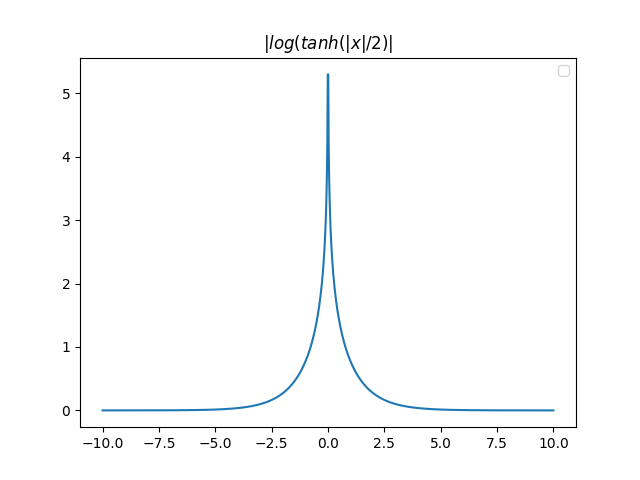
\includegraphics[width=\textwidth]{AWGN/logtanh.png}
		\end{figure}
\end{columns}
For a (3, 2) SPC code, 
\begin{gather*}
    \begin{split}
    f(l_{ext, 1}) & = f(l_2) + f(l_3) \\
    & = f(min(|l_2|, |l_3|))
    \end{split}
\end{gather*}
\begin{gather*}
    \begin{split}
    \Rightarrow |l_{ext, 1}| & = f^{-1}(f(min(|l_2|, |l_3|))) \\
    & = min(|l_2|, |l_3|)
    \end{split}
\end{gather*}
\end{frame}

\begin{frame}{Min-sum approximation for a (n, n-1) SPC code}
Generalising the previously discussed approximation, 
\begin{gather*}
    |l_{ext, n}| = min(|l_1|, |l_2|, ........, |l_{n-1}|)
\end{gather*}
To avoid the repeated computation of sgn() and the minima, we use the folowing procedure.
\begin{gather*}
    S = sgn(l(1) l(2) ....... l(n)) \\
    sgn(l_{ext, i}) = sgn(l_{i}) \times S \\
\end{gather*}
and
\begin{gather*}
    \text{Let }m_1 = min(|l_1|, |l_2|, ........, |l_n|) \\
    pos = argmin(|l_1|, |l_2|, ........, |l_n|) \\
    m_2 = min(|l_1|, |l_2|, ...., |l_{pos-1}|,  |l_{pos+1}|, ...., |l_n|)
\end{gather*}
\end{frame}

\subsection{Algorithm}
\begin{frame}{Decoding Algorithm}
    \begin{itemize}
        \item At $i^{th}$ zero-sum node, 
        \begin{itemize}
            \item Compute the parity $S_i = sgn(m_1)sgn(m_2)...sgn(m_{w_r-1})$.
            \item Compute the absolute value of LLR: 
            \begin{gather*}
                L_i = S_i \times \sum_{j = 1}^{w_r-1}\left|\log(\tanh\left|\frac{m_i}{2}\right|)\right|
            \end{gather*}
        \end{itemize}
        
        \item At $i^{th}$ repetition node, compute $$m_i = r_i + \sum_{j = 1}^{w_c-1} L_i$$
    \end{itemize}
    
Note that there is a slight abuse of notation; the indices 'j' denote the set of edges incident on the particular node.
\end{frame}

\subsection{Algorithm (with min-sum)}
\begin{frame}{Decoding Algorithm with min-sum approximation}
    \begin{itemize}
        \item At $i^{th}$ zero-sum node, 
        \begin{itemize}
            \item Compute the parity $S_i = sgn(m_1)sgn(m_2)...sgn(m_{w_r-1})$.
            \item Compute $pos = argmin(|m_1|, |m_2|, ........, |m_n|)$. \\~\\
                If $ i \neq pos, L_{i} = S_i \times |m_{pos}| $ \\~\\
                Else,  $ L_{i} = S_i \times min(|m_1|, |m_2|, ...., |m_{pos-1}|,  |m_{pos+1}|, ...., |m_n|) $
        \end{itemize}
        
        \item At $i^{th}$ repetition node, compute $$m_i = r_i + \sum_{j = 1}^{w_c-1} L_i$$
    \end{itemize}
    
Note that there is a slight abuse of notation; the indices 'j' denote the set of edges incident on the particular node.
\end{frame}

\subsection{Results}
\begin{frame}
\begin{block}{Terminal output for Belief Propagation}
    \begin{figure}
		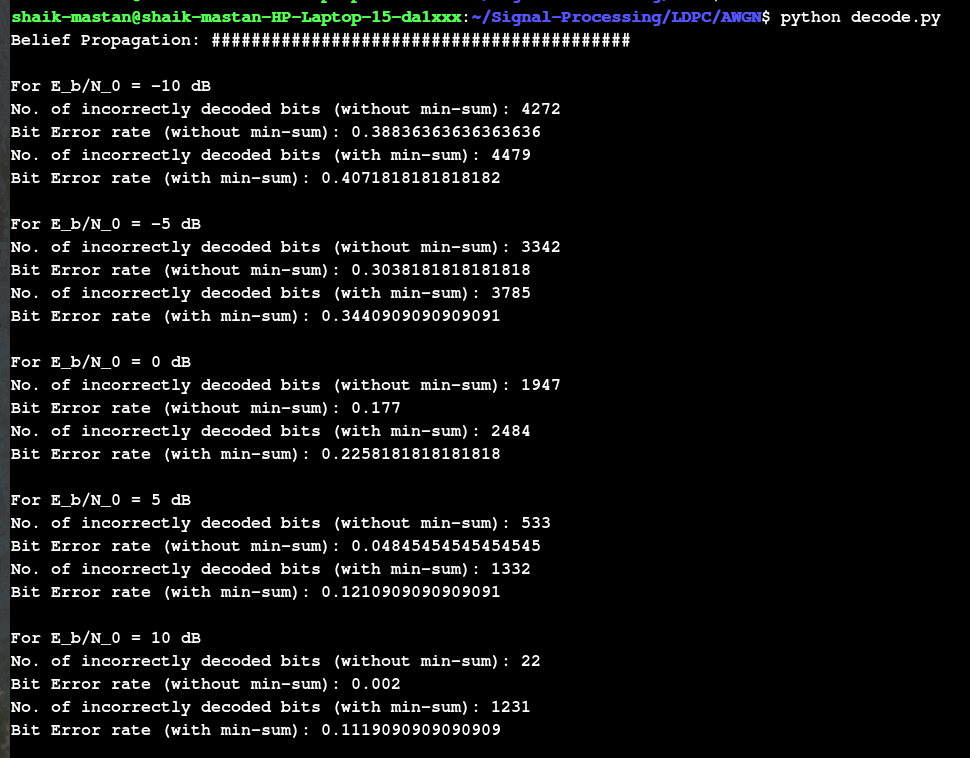
\includegraphics[width=0.8\textwidth]{AWGN/terminalAWGN_1.png}
	\end{figure}
\end{block}
\end{frame}

\begin{frame}
\begin{block}{Terminal output for Gallagher-A}
    \begin{figure}
		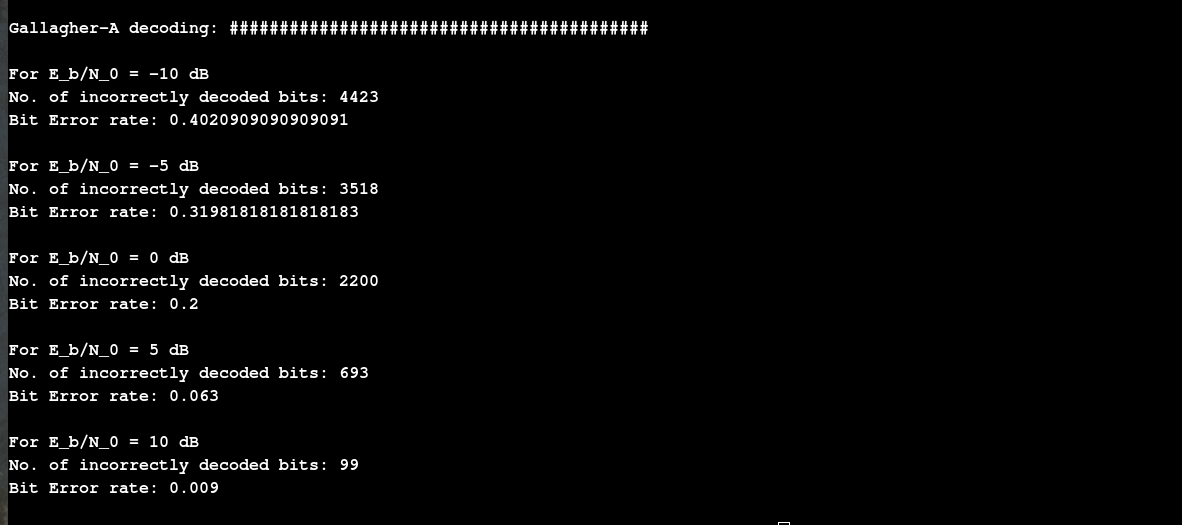
\includegraphics[width=\textwidth]{AWGN/terminalAWGN_2.png}
	\end{figure}
\end{block}

\end{frame}

\begin{frame}
\begin{block}{Comparison with different algorithms}
    \begin{figure}
		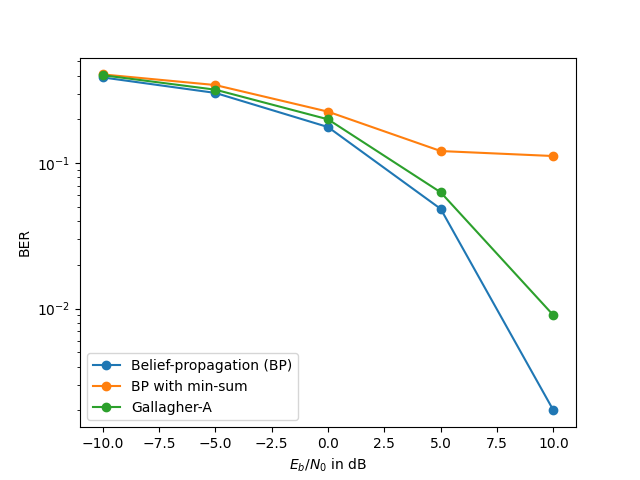
\includegraphics[width=0.8\textwidth]{AWGN/AWGN.png}
	\end{figure}
\end{block}

\end{frame}